\chapter{Basic setup}

\section{Change language}
There are no default languages selected in ArchLinux but the keyboard map is set to 
qwerty\footnote{Most common layout for keyboards} at the beginning. To choose 
your language you have to complete two steps and then the system will be able to 
use it for characters encoding and some softwares as \texttt{nano}.

\subsection{Enable yours}
Before choosing yours it is necessary to enable it in \texttt{/etc/locale.gen}
file with \texttt{locale} tools. 

You will need to use \texttt{nano} to edit the configuration file -- \keys{\ctrl 
+ W} can help you to search -- and remove \og\#\fg{} before the language you want 
to enable (fr\_FR.UTF-8 for example), to save your changes press \keys{\ctrl + X}.
\\
\begin{lstlisting}[language=bash,caption=Enable your language]
$ locale # Current language settings

# Edit the /etc/locale.gen file
$ nano /etc/locale.gen

$ locale-gen # Update available languages
$ locale -a  # See available languages
\end{lstlisting}

\subsection{Change your settings}
The second step is to set the language and configure your keyboard map. 
Notice that you will have to logout for the system to take into account 
changes you made in language setup.
\\ 
\begin{lstlisting}[language=bash,caption=Change language settings]
$ localectl status
  System Locale: n/a  # System language
      VC Keymap: n/a  # Virtual console
     X11 Layout: n/a  # Graphic interface
     
# Change system language (choose enabled one)
$ localectl set-locale LANG=fr_FR.UTF-8

# List of keymaps, choose the one you want "fr-pc" for example
$ localectl list-keymaps

# Change settings 
# no-convert not update VC with X11 and vice versa
$ localectl set-keymap --no-convert fr-pc     # VC Keymap
$ localectl set-x11-keymap --no-convert fr-pc # X11 Layout

# Logout to apply changes
$ exit
\end{lstlisting}

\section{Configure wifi connexion}
\subsection{Check your dongle}
The first thing you can do is checking if your dongle has been recognized by 
the system and can be used.

\begin{lstlisting}[language=bash,caption=Check wifi device]
$ ifconfig -a wlan # All wireless interfaces (also disabled)
\end{lstlisting}

There are a lot of ways to connect your RPi to a network using a wifi dongle 
but all of them requires to install a package before -- wifi-menu needs 
dialog, iw and wpa\_supplicant are not installed -- so it is necessary to 
use an ethernet wire to install them.
\newpage
\begin{lstlisting}[language=bash,caption=Install wireless dependencies]
# pacman is the package manager in ArchLinux
#        -S install a new package 
#
# dialog to get wifi-menu interface
# wpa_supplicant for wireless network protected with wpa keys
#
$ pacman -S dialog wpa_supplicant
\end{lstlisting}

\subsection{Searching the internet}
Once you installed all the packages -- synonym for software -- that wifi-menu 
needed to run you can launch it with \og{}\texttt{wifi-menu}\fg{} command.

\begin{figure}[h]
	\centering
	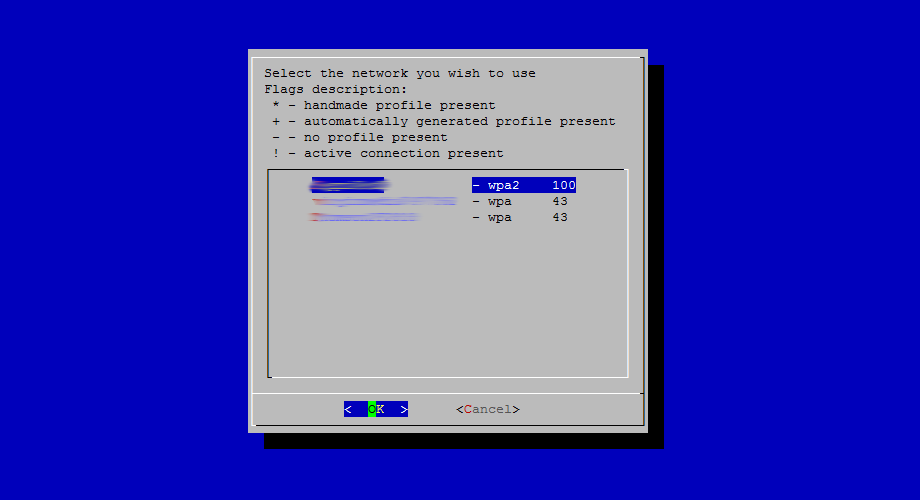
\includegraphics[scale=0.3]{images/WifiMenu.png}
	\caption{wifi-menu interface}
	\label{figure:WifiMenu}
\end{figure}

Then, select your network -- with \keys{\arrowkeyup} and \keys{\arrowkeydown} -- 
, type your password (if required) and you will be connected to your wireless 
network.
\newpage
\section{Create yourself}
\subsection{Simple user}\label{subsec:SimpleUser}
The default username and password for ArchLinux are \texttt{root/root}, this 
user got all right on the system it means he can do anything -- even break the 
system -- so it is not recommanded to use it. 

However, you should change this default password for security purposes and only 
use your new account.
\\
\begin{lstlisting}[language=bash,caption=Create a new user called jeremy]
$ passwd root       # Changes root password (for security)

$ useradd -m jeremy # Creates user jeremy and his home folder
$ passwd jeremy     # Changes jeremy password
\end{lstlisting}

Now we have a new user account for everydays usage. You can see all users on 
your system with \og{}\texttt{cat /etc/passwd}\fg{} which will display the 
content of the config file for users.

\subsection{Very important user}
It is possible to specify user rights with \texttt{visudo} command, the general syntax for one user is 
the following \og{}\texttt{username machine=(targetuser) commands}\fg{}, 
let's look at some details:

\begin{description}
\item[username] name you gave to \texttt{useradd} command
\item[machine] machine on where rights are applied, ALL in general
\item[target user] user that we takes the rights
\item[command] allowed commands separated with one coma -- no spaces --, 
use exclamation mark for banned commands
\end{description}

\texttt{visudo} is the command which prevent you from blocking the system with 
bad changes in the config file \texttt{/etc/sudoers}. The default text editor 
used by \texttt{visudo} is \texttt{vim} but before we used \texttt{nano} so to 
keep using it you have tell it to the system.
\newpage
\begin{lstlisting}[language=bash,caption=Specify user rights]
$ pacman -S sudo   # visudo is inside

# For this session set nano as default editor
# EDITOR is an environement variable
$ export EDITOR=/usr/bin/nano

# To check your changes, use echo which print a message
# in the console and variable with "$" before
$ echo $EDITOR

# Add your account rights after root
# for example "jeremy ALL=(ALL) ALL"
$ visudo
\end{lstlisting}

Now you are a regular user with root permissions but some commands requires
to be root  -- as making changes in systems files -- so if a command want not 
works you can try to add \texttt{sudo} before. 
\\\\
By doing this the system will ask 
you for your password -- even if you are logged -- to get root permissions 
temporarily.

\begin{lstlisting}[language=bash,caption=sudo command usage]
# Logged as jeremy (regular user)
$ visudo
visudo: /etc/sudoers: Permission denied

$ sudo visudo  # Launches visudo with root rights
\end{lstlisting}

This example shows you that \texttt{visudo} command requires to be root so if 
you are logged with a regular account you can not use it. Instead of logout and 
login with root user -- remember do not use this account -- just add 
\texttt{sudo} before your command.

\section{Setup remote connexion}
If you want to keep working with your regular computer on the RPi -- without two 
screens and two keyboards -- it possible to setup a remote connexion with 
\texttt{ssh}\footnote{Remote secure shell access}.
\\\\
On the system there are many programs as \texttt{ssh}  or web server launched 
in background. These programs are regularly started at system startup and 
are called \emph{daemons} or \emph{services}. 
\\\\
Before trying to connect to 
your Raspberry you should check if \texttt{sshd} -- for ssh daemon -- is running.

\begin{lstlisting}[language=bash,caption=Check service state]
$ systemctl status sshd  # Check service state

# If sshd is not running, launch it
$ systemctl start sshd   # Start service

# If after a reboot it is not started
# It can be disabled
$ systemctl enable sshd  # Enable service
\end{lstlisting}

Now that sshd is running, you will be able to connect to it remotely from any 
other system. Here is a list of the methods you should use depending on your own 
machine:

\begin{description}
	\item[Linux and OSX] Use the build-in terminal 
	\item[Windows] PuTTY\footnote{SSH client available on 
					\href{http://www.putty.org}{putty.org}} is the most used 
					tool for this kind of work
\end{description}

Whathever the system you are using, two informations are necessery to perform 
an ssh connexion : remote account --  created in section \ref{subsec:SimpleUser} 
-- and remote machine IP or domain name.

\begin{lstlisting}[language=bash,caption=SSH with command line]
# Format: username@IP (or domain)
$ ssh jeremy@192.168.0.2         # Initiate ssh connexion
jeremy@192.168.0.23's password:  # Type your account password

$ exit  # Stop ssh connexion and go back to local terminal
\end{lstlisting}
